Multiphase flows are ubiquitous in nature and engineering, and their numerical simulation still represents a formidable challenge, especially when a wide range of scales is involved, as in breaking waves on the sea surface, in some industrial processes or in atomizing liquid jets. Scales from meters to microns are typically seen. 
%
% 
Large Reynolds number turbulence, as well as mass and heat transfers
are the main causes for the introduction of such a wide range of scales.
The CO$_2$ transfer and heat exchange between the oceans and the atmosphere is tightly linked to multiphase flows,
as it takes place through the production and dispersion of small bubbles and droplets.
%
Similar small structures are observed in technology, for example in the heat exchange and transport 
in nuclear reactors, the atomization of liquids in combustion and other settings, and in most of the synthesis processes in chemical engineering. For many of these natural and engineering problems, numerical modelling is extremely desirable, albeit a monumental challenge. 

However, in the general area of multiphase flow simulation, much progress has recently been achieved in the interrelated issues of multiple scales, discretization, and topology change. These issues are: i) the long-standing one of how to represent numerically (i.e., simulate) a dynamic or moving curve or surface, ii) the more difficult or challenging problem of how to efficiently model and discretize problems at multiple scales, and finally iii) the still open issue of how to take advantage of hierarchical data structures and grids, such as quadtrees and octrees, to address the ``tyranny of small scales'' \cite{or2018tyranny}. 

The first, moving curve issue is divided into two problems: the kinematic problem, where the motion of the curve or surface separating the phases must be described by knowing the fluid velocity field and the rate of phase change, and the dynamic problem, where the momentum and energy conservation equations must be solved for given fluid properties. Methods available for the kinematic problem are sometimes separated into Front-Capturing and Front-Tracking methods. In the first kind, Front-Capturing methods, a tracer or marker function $f(\X,t)$ is integrated in time with the knowledge of an adequate velocity field
$\U(\X,t)$
\be
\dert f + \U \cdot \nabla f = 0
\nd
The tracer function can be a Heaviside function, leading to Volume-of-Fluid (VOF) methods \cite{Hirt_1981_39, Brackbill_1992_100} or a smooth function, leading to Level-Set (LS) methods \cite{Osher_1988_79, Osher_2001_169}.

In Front-Tracking methods, the interface or ``front'' is represented by a curve discretization, for example a spline, which evolves with a
prescribed normal velocity $V_S$ , see \cite{Unverdi_1992_100}. Compatibility between the two formulations is achieved if $\U \cdot \N = V_S$. An introduction to the most
popular methods may be found in \cite{Tryggvason_2011_book}. Another point of view on the methods, that is fruitful in connection with
issues ii) and iii) above, can be obtained by investigating how the data
structures are tied to the underlying Eulerian grid. The  data structures are {\em local} when
their components have little or no ``knowledge'' of the
overall connections among pieces of interface or connected regions of a given phase (Fig.~\ref{Fig_GT}b). Thus a discretization of the tracer function $f$ is a local
data structure, tied to the Eulerian grid. On the other hand a {\em global data structure} contains information not only about individual points on the interface, but also about
their connections with the entire interface of a given object. For Front-Tracking methods this is achieved by linked lists, or pointers, that
allow to navigate the data structure along the object (Fig.~\ref{Fig_GT}a). It is then obvious and efficient, using the data structure, to find all the connected pieces of the interface.
% ----------
\begin{figure}
\begin{center}
\begin{tabular}{cc}
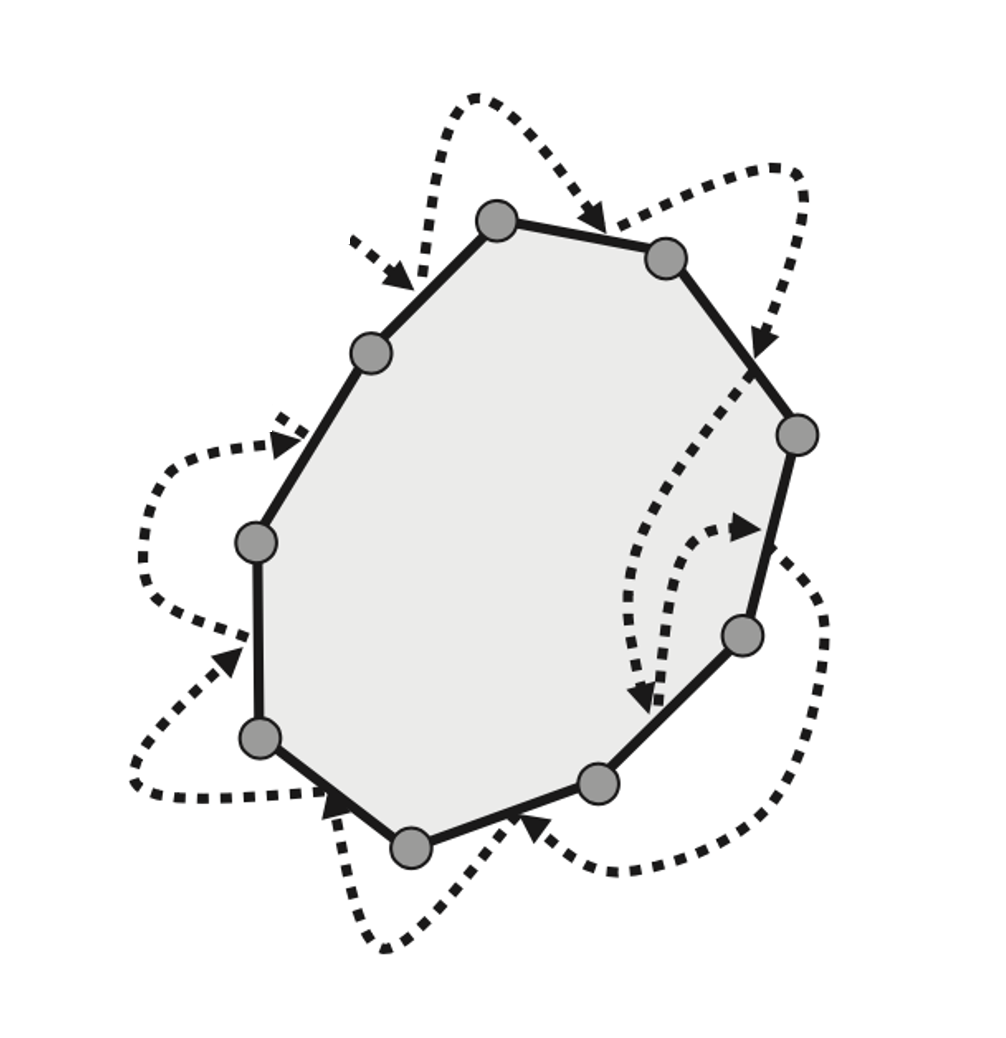
\includegraphics[width=0.45\textwidth]{linked} &
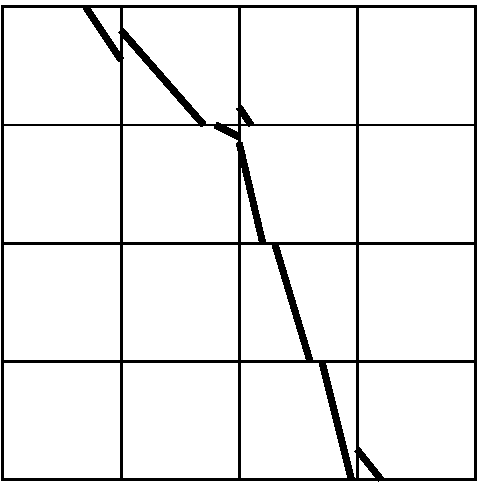
\includegraphics[width=0.4\textwidth]{vof}\\
(a) & (b) 
\end{tabular}
\end{center}
\caption{(a) A global data structure with a linked list: the example of the front. Reproduced from \cite{Tryggvason_2011_book}; (b) A local data structure with unlinked VOF linear reconstructions.}
\label{Fig_GT}
\end{figure}
% ----------
The local data structures are not limited to VOF or LS methods. For example, an unconnected marker or particle method, such as Smoothed Particle Hydrodynamics (SPH), or other methods, simply tracks particles of position ${\bf x}_i$ by integrating
\be
\romandt{\X_i} = \U(\X_i,t)
\nd
without any concept of connection between the particles \cite{chen1997surface}. Such an unconnected marker method, despite its similarity with Front-Tracking is in fact a {\em local} method. 
Both the local and the global approaches have advantages. The local methods are easy to parallelize on a grid, are free of constraints that require the solutions of large linear or nonlinear systems (as when constructing interfaces by high-order splines) and are generally computationally efficient. The global methods allow to track and control the topology, so they are also useful for the second issue, the handling of multiscale problems.
Moreover, when dealing with complex multiscale problems, it is often useful to investigate geometrical properties such as skeletons \cite{chen2022characterizing} which are branched manifolds most naturally represented by Front-Tracking. 
Global methods also allow to naturally distinguish between continuous slender objects such as unbroken thin ligaments or threads and strings of small particles or broken ligaments. This latter distinction is of great importance when analyzing statistically highly-fragmented flows \cite{Chirco_2022_467}. 
It is however possible to represent slender objects with local methods in some case. Chiodi \cite{Chiodi_2020_phd} proposed an enhancement of the VOF reconstruction: the reconstruction with 2-planes (R2P) method. The method considers two planes with arbitrary relative orientation, a feature that allows the modelling of sub-grid scale thin sheets, the closure of sheet rims and in general a more accurate sub-grid interface reconstruction. 
The moment-of-fluid (MOF) method \cite{Shashkov_2023_479, Shashkov_2023_494} first proposed by 
Dyadechko and Shashkov \cite{Dyadechko_2008_227}, in which the zeroth, first and second moments of the fragment of material inside a cell are used for interface reconstruction by one half-plane, two half-planes or a circle, is also able to exactly capture corners, filaments and some concave shapes smaller than the grid spacing.
A method that combines some of the properties of global methods, such as Front-Tracking, and of local ones, such as VOF or LS,
seems desirable. There have been indeed some prior attempts at such a combination.

Aulisa et al. \cite{Aulisa_2003_188, Aulisa_2004_197} combined the VOF method with marker points to obtain smooth
interfaces without discontinuity and to improve mass conservation of traditional Front-Tracking methods. L\'{o}pez et al. \cite{Lopez_2005_208} introduced marker points into the VOF method to allow the tracking of fluid structures thinner than the cell size.

The Level Contour Reconstruction Method (LCRM) developed by Shin, Juric and collaborators \cite{Shin_2002_180, Shin_2005_203, Shin_2007_21} combined Front-Tracking and LS methods. It improved the mass conservation problem of traditional LS methods, thanks to the tracking of the interface by Lagrangian elements (instead of advecting the LS function field).
%
A LS function can then be generated from the Lagrangian elements.
%
The smoothing of interface elements, as well as topology changes, take place automatically during the reconstruction procedure, thus explicit connectivity information is not needed in their method. Singh and Shyy \cite{Singh_2007_224} used the LCRM to perform topology changes in their traditional Front-Tracking method where connectivity of the Lagrangian elements has to be maintained explicitly.
%
Shin, Yoon and Juric \cite{Shin_2011_230} later extended the LCRM to obtain a new type of Front-Tracking method, the Local Front Reconstruction Method (LFRM), for both two-dimensional and three-dimensional multiphase flow simulations. The LFRM reconstructs interface elements using the geometrical information directly from the Lagrangian interface elements instead of constructing another LS field.

We suggest a similar method in the present work, based on a purely kinematic approach 
developed by two of us \cite{Chirco_2022_95},
called the Edge-Based Interface-Tracking (EBIT) method.
%
In that method the position of the interface is tracked by marker points
located on the edges of an Eulerian grid, and 
the connectivity information is implicit.
%
The basic idea and the split interface advection were discussed in \cite{Chirco_2022_95},
here we improve the mass conservation of the original EBIT method by using a circle fit to reconstruct the interface during advection.
%
A topology change mechanism is also introduced.
Compared to the LFRM of Shin, Yoon and Juric \cite{Shin_2011_230}, markers in the EBIT method are bound to the
Eulerian grid. These marker are obtained by a reconstruction of
the interface at every time step, thus the Eulerian grid and Lagrangian markers can be distributed to different processors by the same routine
as the one used in the parallelization of the Navier--Stokes solver.
Second, a new feature called Color Vertex,
which amounts to describe the topology of the interface by the color of
markers at the vertices of the grid, is discussed. 
Such a scheme is trivial on a simplex and just slightly more complicated on a square grid. It was
proposed in a similar context by Singh and Shyy \cite{Singh_2007_224}.
Third, we combine the EBIT method with a Navier--Stokes solver for multiphase flow simulations. The coupling is simply
realized by computing volume fractions from the position of the markers and the Color Vertex, then we use the volume fractions as in typical VOF solvers \cite{Tryggvason_2011_book}. 

The paper is organized as follows: the kinematics of the EBIT method is described in Section \ref{Numerical method}.
This includes the interface advection algorithm, the updating rules for the Color Vertices and the automatic topology change algorithm.
Then the coupling algorithm between the EBIT interface description and the multiphase fluid dynamics is presented. 
A two-dimensional flow solver based on a Cartesian or quadtree grid is implemented inside the free platform Basilisk \cite{Popinet_2003_190, Popinet_2009_228}. In Section \ref{Numerical results and discussion}, the EBIT method is validated by the computation of typical examples of
multiphase flow simulations. 
The results obtained by the combined EBIT method and Navier--Stokes solver are presented and compared with those calculated by the PLIC-VOF method implemented inside Basilisk \cite{Popinet_2009_228}.
